%--------------------------------------------------------------------------------------------------
\chapter{Stand der Technik}\label{cha:StandDerTechnik}

In diesem Kapitel gibt es einen Einblick in die Themenbereiche Industrie 4.0, industrielle Fertigung, und Virtual Reality.
\newline
Zunächst wird der Begriff Industrie 4.0 definiert, bevor auf die Geschichte der industriellen Revolutionen der vergangenen 260 Jahre sowie die Veränderungen in der Informations- und Kommunikationstechnik eingegangen wird. Außerdem gibt es einen Einblick in die Potenziale und Herausforderungen von Industrie 4.0, bevor zwei Leitfaden für die Umsetzung von Industrie 4.0 in Unternehmen vorgestellt werden.
Daraufhin gib es einen Einblick in die Ausgangslage der industriellen Fertigung, insbesondere in den Produktlebenszyklus, die Automatisierungspyramide und ihren Wandel im Kontext von Industrie 4.0.
Zum Schluss wird das Thema Virtual Reality (VR) vorgestellt, daher gibt es einen Einblick in die Geschichte und die Potenziale von Virtual Reality.

%--------------------------------------------------------------------------------------------------
\section{Industrie 4.0}\label{sec:Industrie4.0}
Erstmalig tauchte der Begriff Industrie 4.0 auf der Hannover Messe 2011 auf und wurde daraufhin ein zentraler Bestandteil der Hightech-Strategie der deutschen Bundesregierung \cite{8}.
\newline
Der Begriff Industrie 4.0 „steht für die 4. Industrielle Revolution, einer neuen Stufe der Organisation und Steuerung der gesamten Wertschöpfungskette über den Lebenszyklus von Produkten“ \cite{1}. Dies führt zum einen zu einer zunehmenden Vernetzung von „Mensch, Maschinen und Werkstücken durch Modernste Informations- und Kommunikationstechnik“ \cite{6}, zum anderen auch zu einer zunehmenden „Vernetzung der realen mit der virtuellen Welt“ \cite{7}.
\newline
Grundlage dieser Wandlung in der Industrie sind sogenannte Cyber-Physische-Systeme (CPS), also moderne Steuerungssysteme mit eingebetteten Softwaresystemen und Anbindung an das Internet \cite{1}. Cyber-Physische-Systeme verknüpfen „reale (physische) Objekte und Prozesse mit informationsverarbeitenden (virtuellen) Objekten und Prozessen“ \cite{11}. Dies hat eine zunehmende Verschmelzung von Fertigungsprozessen und Informationstechnologie zur Folge \cite{7}.

\subsection{Industrielle Revolution und Informations- und Kommunikationstechnik}\label{sec:GeschichteIndustrie4}
Um den Begriff Industrie 4.0 besser nachvollziehen zu können, ist es unumgänglich die Geschichte der industriellen Revolutionen der vergangenen 260 Jahre zu verstehen. Der Begriff Industrie 4.0 „leitet sich aus den großen Industriegeschichtlichen Umbrüchen ab“ \cite{7} und ist ein Wortspiel aus den Anteilen „Industrie“ und „4.0“. Der Anteil „4.0“ soll zum einem eine Assoziation zum Internet (Web 4.0) herstellen und zum anderen eine Versionsbezeichnung darstellen, wie man sie beispielsweise aus dem Bereich der Softwareentwicklung kennt \cite{1}.
\newline
Industrie 4.0 wird als „der vierte große technologische Durchbruch“ \cite{7} betrachtet. Daher werden im Folgenden die industriellen Revolutionen bis zur Industrie 4.0 und die Entwicklung der Informations- und Kommunikationstechnik bis Web 4.0 betrachtet.
\newpage

\subsubsection{Die industriellen Revolutionen}\label{sec:IndustrielleRevolution}
\begin{figure}[h]
	\centering
	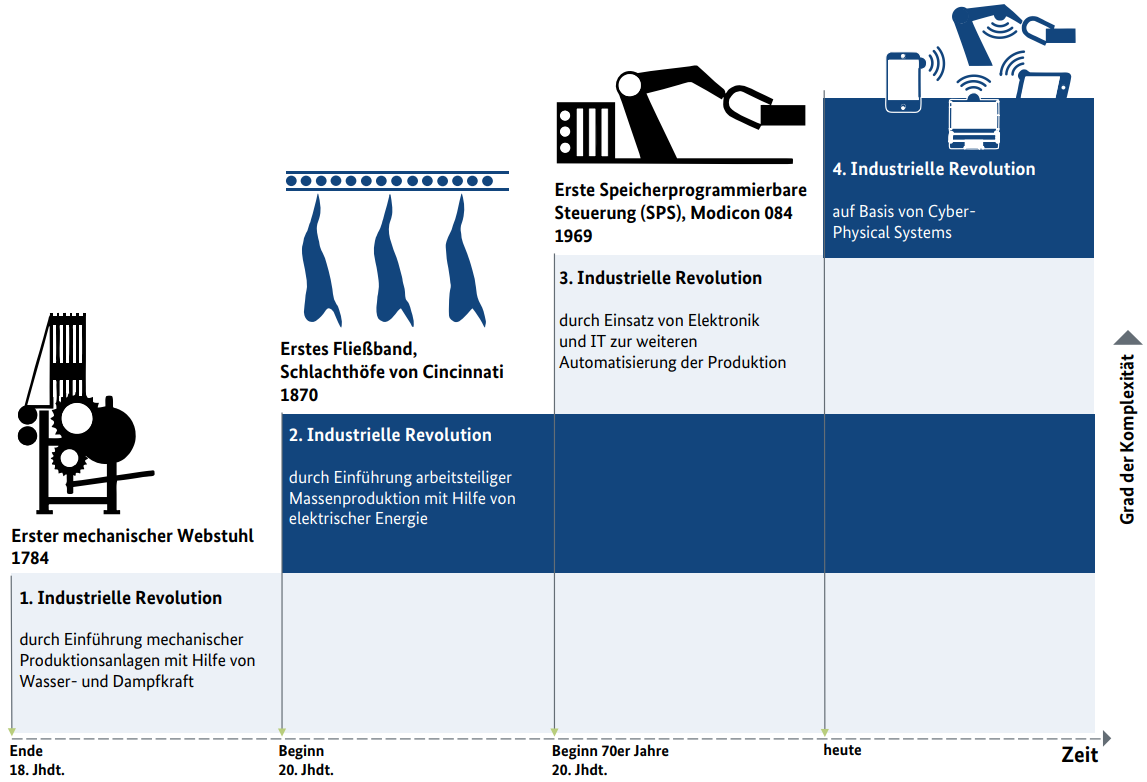
\includegraphics[width=1\linewidth]{Bilder/A1_DieGeschichteDerIndustriellenRevolutionenBMWI}
	\caption{Die Geschichte der Industriellen Revolutionen \cite[S.8]{A1}}
	\label{fig:IndustrielleRevolutionenBild}
\end{figure}
\FloatBarrier
\noindent Die \textbf{erste industrielle Revolution} spielte sich Mitte bis Ende des 18. Jahrhunderts ab. Im Fokus standen Wasser- und Dampfkraft, was die Möglichkeit mit sich brachte Maschinen die vorher noch mit menschlicher Kraft angetrieben wurden mithilfe von Wasser- und Dampfkraft anzutreiben. Die Menschen erkannten früh, dass sich durch die neuen industriellen Entwicklungen eine große Menge an Arbeitsplätzen schaffen lassen können. \cite{9}. Neben gesteigerter Produktivität in der Herstellung führte die erste industrielle Revolution dazu, „dass seit dieser Zeit in industriell geprägten Ländern keine strukturell bedingten Hungerkatastrophen mehr entstanden sind“ \cite[S.5]{15}. Des Weiteren führte die verbesserte Infrastruktur durch Dampfschiffe und Eisenbahnen zu einer besseren Kleidungs- und Nahrungsversorgung und zu einem enormen Bevölkerungswachstum \cite[S.5]{15}. Außerdem gab es große Auswirkungen auf die Gesellschaft, da zwei neue Schichten in der Bevölkerung entstanden: die Fabrikarbeiterschaft und die Fabrikbesitzer \cite[S.5]{15}. Die Entwicklungen der ersten industriellen Revolution brachten allerdings einige große Probleme mit sich. Dazu gehören Beispielsweise die Ausbeutung der Fabrikarbeiter durch schlechte Arbeitsbedingungen und Bezahlung, Kinderarbeit und sogar eine verkürzte Lebenserwartung für die Fabrikmitarbeiter \cite[S.5]{15}.
\newline\newline
Die \textbf{zweite industrielle Revolution} zu Beginn des 20. Jahrhunderts „war geprägt durch arbeitsteilige Massenproduktion mit Hilfe elektrischer Energie“ \cite[S.5]{15}. Ermöglicht wurde die Massenproduktion unter anderem durch das von Henry Ford entwickelte Fließband, welches bereits 1913 in der Automobilproduktion eingesetzt wurde \cite{10}. Des Weiteren führten die Entwicklungen von elektrischen Antrieben und Verbrennungsmotoren zu einer zunehmenden Dezentralisierung. Dezentralisierung im Kontext der zweiten industriellen Revolution bedeutet, „die Arbeitsmaschinen nicht durch zentrale Kraftmaschinen anzutreiben, sondern dezentral zu betreiben“ \cite[S.6]{15}. Ein weiterer „Erfolgsfaktor in der zweiten industriellen Revolution waren die ersten Schritte der Globalisierung“ \cite{9} durch die Fortschritte in der Verkehrsinfrastruktur. Dazu gehören Beispielsweise moderne Schiffe, die eine bessere Vernetzung zwischen den Kontinenten ermöglicht haben \cite{9}. Für die Chemie- und Automobilindustrie wurde Erdöl zu einem wichtigen Rohstoff. „Die großindustrielle Massenproduktion“ \cite[S.6]{15} ermöglichte die Produktion von immer günstigeren (Konsum-)Gütern für die weiterhin wachsende Bevölkerung \cite[S.6]{15}. Die Gesellschaft erkannte, dass die Ausbeutung der Fabrikarbeiter nicht weiter gehen kann und Gewerkschaften gewannen stark an Bedeutung. Daher sollten Fabrikarbeiter von nun an besser entlohnt werden, um weitere soziale Spannungen zu vermeiden \cite[S.6]{15}. Im Übergang zwischen der ersten und zweiten industriellen Revolution verbreiteten sich die Ideen des Kommunismus und der Sozialdemokratie \cite[S.6]{15}.
\newline\newline
Die \textbf{dritte industrielle Revolution} Mitte des 20. Jahrhunderts wurde geprägt durch zunehmende Automatisierung der Produktionsabläufe durch das einbinden von Elektronik und Informations- und Kommunikationstechnik \cite[S.7]{15}. Durch den Einsatz von programmierbaren Steuerungen, „waren auch in den Fabriken Programmierer gefragt“ \cite{10}. Des Weiteren wurde der Personal-Computer (PC) vermehrt im Büro aber auch im Haushalt eingesetzt \cite{9}. Die Entwicklungen der dritten industriellen Revolution ermöglichten eine variantenreiche Serienproduktion. Mit dieser Entwicklung veränderten sich aber auch die Erwartungen der Kunden, welche nun vermehrt auf Individualität und Qualität der Produkte achteten \cite[S.7]{15}.
\newline\newline
Die \textbf{vierte industrielle Revolution} ist momentan noch im Gange. In Kapitel \ref{sec:PotentialeIndustrie4.0} und \ref{sec:HerausforderungenUmsetzung} gibt es einen Einblick in die Potentiale und Herausforderungen von Industrie 4.0. Vorweg lässt sich aber sagen, dass die vierte industrielle Revolution die Industrie flexibler gestalten soll, statt ein höheres Grad an Automatisierung zu erreichen. Die Wertschöpfung soll durch Cyber-Physische-Systeme verbessert werden. Es ist wichtig zu wissen, dass die Entwicklungen der Industrie 4.0 aus zwei Entwicklungsrichtungen kommen \cite{1}:
\begin{enumerate}
	\item \textbf{„Physicalize the Cyber"} \cite{1} \\ Aus der Sicht der informationstechnischen Unternehmen: „Zunehmende Nutzung von Informationstechnik in der Produktion“ \cite{1}.
	\item \textbf{„Cyberize the Physical"} \cite{1} \\ Aus der Sicht der produktionstechnischen Unternehmen: „Anwendungen für Informationstechnik in der Produktion“ \cite{1}.
\end{enumerate}

\subsubsection{Informations- und Kommunikationstechnik}\label{sec:WebRevolution}
Genauso wie in der Industrie gab es in der Informations- und Kommunikationstechnik einige technologische Umbrüche. Auffällig ist, dass sich die Technologien der Informations- und Kommunikationstechnik im Vergleich zu den Fortschritten in der Industrie sehr schnell weiterentwickeln. Daher steht die Industrie vor der Aufgabe mit diesen schnellen Entwicklungen Schritt zu halten. Die wichtigsten Umbrüche sind in der Abbildung \ref{fig:WebRevolutionBild} zusammengefasst. Wie man der Abbildung \ref{fig:WebRevolutionBild} entnehmen kann, stehen in der neuen Entwicklungsstufe von Informations- und Kommunikationstechnik Cyber-Physische Medien im Mittelpunkt.
\begin{figure}[h]
	\centering
	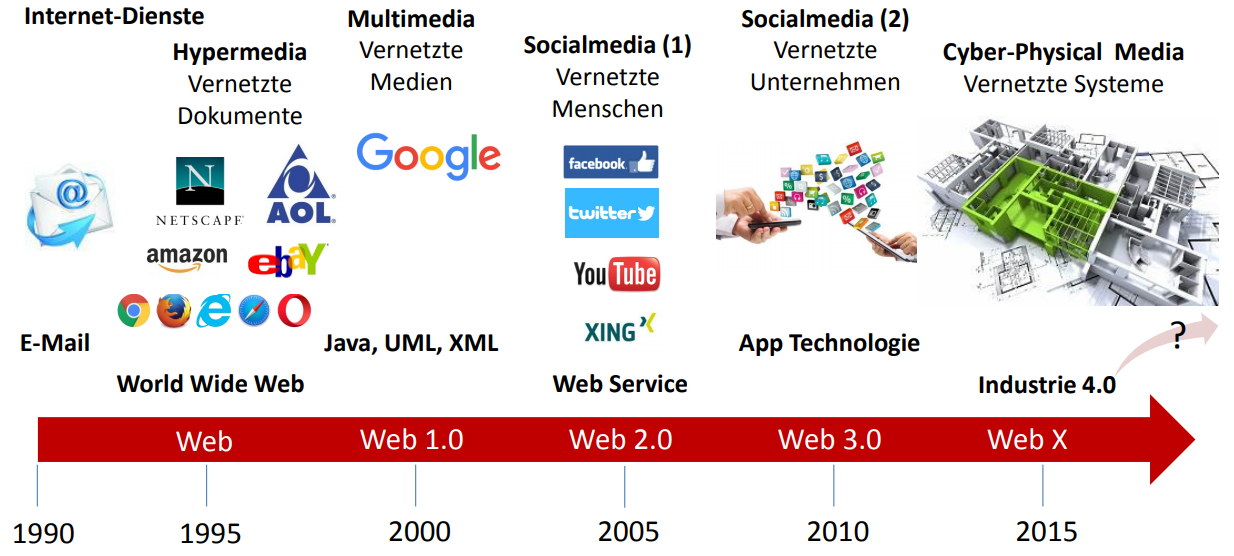
\includegraphics[width=1\linewidth]{Bilder/A2_EntwicklungWeb0-4}
	\caption{Die Entwicklung von Web bis Web 4.0 \cite{A2}}
	\label{fig:WebRevolutionBild}
\end{figure}

\subsection{Potentiale von Industrie 4.0}\label{sec:PotentialeIndustrie4.0}
„Industrie 4.0 macht die Produktion individueller und effizienter“ \cite{6}, ermöglicht durch das Vernetzen von „Mensch, Maschinen und Werkstücken durch modernste Informations- und Kommunikationstechnik“ \cite{6}. Dies verspricht dem Wirtschaftsstandort Deutschland Wachstumschancen und sogar Wettbewerbsvorteile bei entsprechender Umsetzung. Laut dem Bundesverband der Deutschen Industrie (BDI) prognostizieren Experten eine Produktivitätssteigerung von bis zu 30 Prozent bis zum Jahr 2025 \cite{6}.
\newline
Mit Industrie 4.0 sollen nicht nur große Unternehmen, sondern gezielt auch der Mittelstand angesprochen werden, um ihm wirtschaftlichen Nutzen bringen, da dieser das Rückgrat der deutschen Industrie bildet. Laut einer Studie der Commerzbank haben 86 Prozent der Unternehmen die Potentiale von Industrie 4.0 erkannt, zögern aber noch mit der Einführung \cite[S.4]{2}. Man kann sogar sagen, dass sich dem deutschen Mittelstand durch neuartige und innovative Produkte die Möglichkeit eröffnet, den Wandel zu Industrie 4.0 aktiv mitzugestalten \cite[S.8]{2}. Dennoch gibt es viele Unternehmen, denen „der konkrete Nutzen von Lösungsansätzen im Umfeld von Industrie 4.0 nicht ersichtlich“ ist \cite[S.7]{2}. 
\newline
Der Bundesverband der Deutschen Industrie e.V. hat die Unternehmensberatung Roland Berger mit einer „Studie zur digitalen Transformation der Industrie“ \cite{8} beauftragt. Die Studie kam zu dem Ergebnis, dass beim Verpassen der aktuellen Entwicklungen dem Wirtschaftsstandort Deutschland „Einbußen bei der industriellen Wertschöpfung bis 2025 von insgesamt 220 Milliarden Euro“ \cite{8} drohen. Europaweit rechnet man sogar mit Einbußen von bis zu 605 Milliarden Euro. Bei einem erfolgreichen Anknüpfen an den Wandel zu Industrie 4.0 „prophezeit die Studie der Automobilindustrie schon im Jahr 2025 ein sattes Wertschöpfungsplus von 35 Milliarden Euro“ \cite{8} und dem Maschinen- und Anlagebau sogar bis zu 89 Milliarden Euro. Die Studie der Unternehmensberatung Roland Berger kam weiterhin zu dem Ergebnis, dass sich 55 Prozent der befragten Unternehmen „bereits intensiv mit der digitalen Transformation“ \cite{8} beschäftigt haben, aber 43 Prozent die Bedeutung der Digitalisierung und des Wandels hauptsächlich in der Kostenreduktion sieht \cite{8}. Des Weiteren schätzen sich rund ein Drittel der Unternehmen als hoch oder sehr hoch digitalisiert ein. Bei profitablen Unternehmen liegt dieser Anteil sogar bei 62 Prozent \cite{8}.
\newline
Im Folgenden sind vielversprechende Potentiale von Industrie 4.0 zusammengefasst:
\begin{enumerate}
	\item \textbf{„Individualisierung der Kundenwünsche"} \cite[S.19]{12} \\
	Ermöglicht Rücksicht auf individuelle Kundenwünsche zu nehmen. Dabei bleibt die 
	Produktion selbst bei Bestellungen von Einzelstücken oder Kleinstmengen (Losgröße 1) 
	effizient und rentabel \cite[S.19]{12}.
	\item \textbf{„Flexibilisierung"} \cite[S.20]{12} \\
	Optimierungen „in unterschiedlichen Dimensionen: Qualität, Zeit, Risiko, Robustheit, Preis,
	Umweltverträglichkeit, etc.“ ermöglicht es die Produktionsprozesse flexibel zu gestalten,
	kurzfristig zu verändern und auf unerwartete Ausfälle zu reagieren \cite[S.20]{12}.
	\item \textbf{„Optimierte Entscheidungsfindung"} \cite[S.20]{12} \\
	Durch das Sammeln von produktionstechnisch relevanten Daten in Echtzeit fällt es leichter
	die (richtigen) Entscheidungen zu treffen, um auf Störungen zu reagieren, eine
	„standortübergreifende globale Optimierung“ durchzuführen und auf dem globalen Markt 
	wettbewerbsfähig zu bleiben \cite[S.20]{12}. Daher sollte die Vernetzung der 
	Unternehmen nicht nur firmenintern und lokal, sondern auch Unternehmens übergreifend 
	(z.B. mit Zulieferern/Kunden) stattfinden \cite{6}.
	\item \textbf{„Ressourcenproduktivität und Effizienz"} \cite[S.20]{12} \\
	„Smart Factorys“, also Fabriken mit Produktionsanlagen die sich eigenständig und in Echtzeit 
	koordinieren und optimieren und somit die Produktion effizienter und flexibler gestalten \cite{6}. Dabei wird bei gleichbleibendem oder sogar niedrigerem 
	Ressourceneinsatz die Produktionsmenge gesteigert \cite[S.20]{12}.
	\item \textbf{„Wertschöpfungspotenziale durch neue Dienstleistungen"} \cite[S.20]{12} \\
	Es eröffnet sich ein neuer Markt für innovative Dienstleistungen, vorangetrieben durch die
	gesammelten Daten über den gesamten Lebenszyklus von intelligenten Produkten 
	\cite[S.20]{12}. Durch das „Internet der Dinge“ (Internet of Things, kurz: IOT)
	werden intelligente Produkte zu Dienstleistungen, sogenannten „Smart Services“, da sie 
	während Ihrer gesamten Lebensdauer mit dem Internet verbunden sind \cite{6}.
	\item \textbf{„Demografie-sensible Arbeitsgestaltung"} \cite[S.20]{12} \\
	Die Unternehmen bekommen durch verbesserte Arbeitsbedingungen die Chance auf den 
	demographischen Wandel zu reagieren und sogar davon profitieren zu können \cite[S.20]{12}. Durch den Fachkräftemangel und die alternde Bevölkerung ist es wichtig 
	„ältere Menschen länger in das Berufsleben einzubinden“ \cite{6}.
	\item \textbf{„Work-Life-Balance"} \cite[S.20]{12} \\
	Intelligente Assistenzsysteme helfen dabei, „den Arbeitseinsatz so zu gestalten, dass sowohl
	den Flexibilitätsbedürfnissen der Betriebe als auch den notwendigen Flexibilitätsspielräumen
	für den privaten Bereich in neuer Qualität Rechnung getragen werden kann“ \cite[S.20]{12}. Diese Assistenzsysteme können unterschiedlich aussehen. Einige Beispiele dafür sind mobile Geräte wie Tablet Computer oder Virtual/Augmented Reality Brillen \cite{6}.
	\item \textbf{„Wettbewerbsfähigkeit als Hochlohnstandort"} \cite[S.20]{12} \\
	Deutschland gilt als ein Hochlohnstandort. Um auf den internationalen Markt 
	wettbewerbsfähig zu sein müssen die Unternehmen genug erwirtschaften um profitabel
	zu sein. Industrie 4.0 gibt Unternehmen die Chance eine lohnenswerte Produktion im eigenen Land zu betreiben \cite[S.20]{12}.
	\item \textbf{„Smart Products"} \cite{6} \\
	Intelligente Produkte mit integrierten Chips (z.B. RFID Chips) liefern selbst alle benötigten
	Informationen für die Produktion. So kann Beispielweise ein Produkt einer Maschine 
	mitteilen in welcher Farbe es lackiert werden soll. Des Weiteren liefern diese Chips Daten, 
	welche für das virtuelle Abbild des Produktes und der Produktion genutzt werden. \cite{6}.
	\item \textbf{„Simulation und Überwachung der Produktion"} \cite{6} \\
	Durch einen digitalen Zwilling und die Sammlung von Daten in Echtzeit kann die gesamte
	Produktion simuliert und überwacht werden. Dies ermöglicht Beispielsweise die
	Fernsteuerung, Simulation und Überwachung der Produktion in Echtzeit \cite{6}.
	\item \textbf{„Chancen für IT-Unternehmen"} \cite[S.7]{2} \\
	Es eröffnen sich immer mehr Chancen für Unternehmen aus dem Bereich der Informations- und Kommunikationstechnik in produktionstechnisch geprägten Märkten Fuß zu fassen \cite[S.7]{2}.
\end{enumerate}

\subsection{Herausforderungen bei der Umsetzung}\label{sec:HerausforderungenUmsetzung}
Der Wandel zu Industrie 4.0 bringt viele neue Herausforderungen mit sich, da es für den Wandel keinen allgemein anwendbaren Lösungsweg gibt. Wie in Abbildung \ref{fig:HerausforderungenIndustrie4.0} illustriert gibt es im Folgenden einen Einblick in die fünf wichtigsten Herausforderungen nach Roth \cite{14} die der Wandel zu Industrie 4.0 mit sich bringt.
\begin{figure}[h]
	\centering
	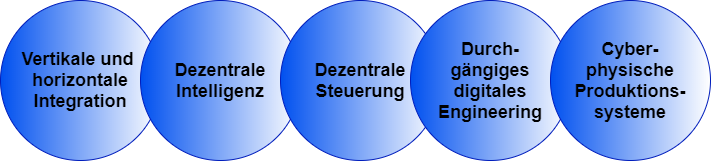
\includegraphics[width=1\linewidth]{Bilder/A11_HerausforderungenIndustrie4}
	\caption{Herausforderungen von Industrie 4.0, Abbildung nach \cite[S.37]{14}}
	\label{fig:HerausforderungenIndustrie4.0}
\end{figure}

\subsubsection{Horizontale und Vertikale Integration}\label{sec:HorizontaleVertikaleIntegration}
Die \textbf{horizontale Integration} (Abbildung \ref{fig:HorizontaleIntegration}) in der Produktions- und Automatisierungstechnik und der IT erfordert "die Integration der verschiedenen IT-Systeme für die unterschiedlichen Prozessschritte der Produktion und Unternehmensplanung, zwischen denen ein Material-, Energie- und Informationsfluss verläuft" \cite[S.24]{12}. Das Ganze muss sowohl unternehmensintern (Logistik, Fertigung, etc.), als auch unternehmensübergreifend (Zulieferer, Produzenten, etc.) stattfinden, um eine durchgängige Lösung zu ermöglichen \cite[S.24]{12}.
\begin{figure}[h]
	\centering
	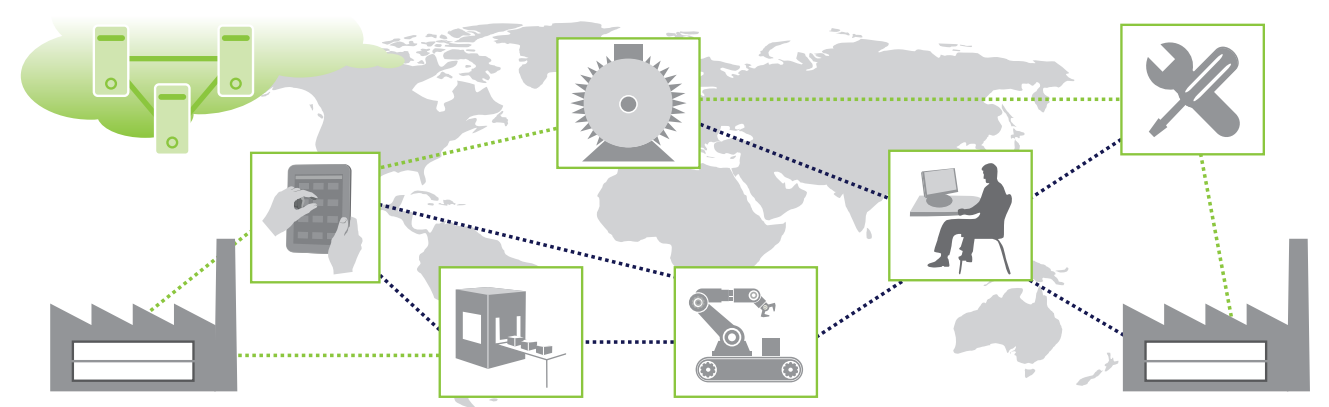
\includegraphics[width=0.7\linewidth]{Bilder/A3_HorizontaleIntegration}
	\caption{Schaubild horizontale Integration \cite[S.35]{12}}
	\label{fig:HorizontaleIntegration}
\end{figure}
\newline
\noindent Die \textbf{vertikale Integration} (Abbildung \ref{fig:VertikaleIntegration}) in der Produktions- und Automatisierungstechnik und der IT erfordert "die Integration der verschiedenen IT-Systeme auf den unterschiedlichen Hierarchieebenen (beispielsweise die Aktor- und Sensorebene, Steuerungsebene, Produktionsleitebene, Manufacturing and Execution-Ebene, Unternehmensplanungsebene)" \cite[S.24]{12} um eine durchgängige Lösung zu ermöglichen \cite[S.24]{12}.
\begin{figure}[h]
	\centering
	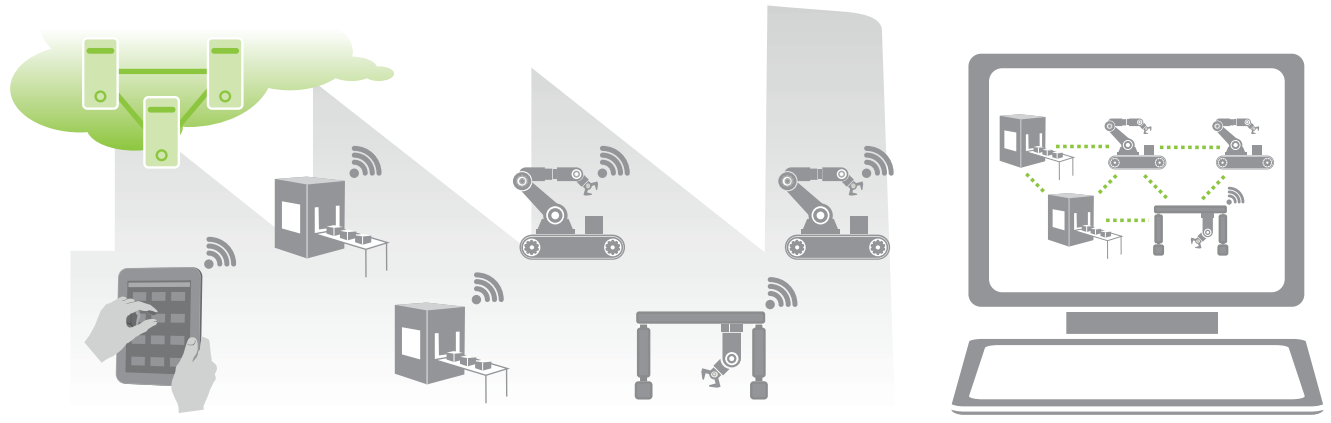
\includegraphics[width=0.7\linewidth]{Bilder/A4_VertikaleIntegration}
	\caption{Schaubild vertikale Integration \cite[S.36]{12}}
	\label{fig:VertikaleIntegration}
\end{figure}

\subsubsection{Dezentrale Intelligenz}\label{sec:DezentraleIntelligenz}
Dezentrale Intelligenz ermöglicht „Produktionsmitteln und -anlagen individuell und ortsunabhängig für den Produktionsprozess relevante Informationen an ein dezentrales Steuerungssystem weitergeben zu können“ \cite[S.39]{14}. Daher bildet die dezentrale Intelligenz das Fundament für die dezentrale Steuerung. 
Für die Realisierung von dezentraler Intelligenz bedarf es auf der Produktseite Produkte mit eingebetteten RFID-Chips und auf der Produktionsseite Produktionssysteme mit entsprechenden Sensoren und Computersystemen zum Verarbeiten der ausgelesenen Daten \cite[S.39]{14}.

\subsubsection{Dezentrale Steuerung}\label{sec:DezentraleSteuerung}
Es findet eine Entwicklung „weg von einer ortsgebundenen, unflexiblen Steuerung“ \cite[S.40]{14} statt. Dezentrale Systeme und das Internet der Dinge und Dienste ermöglichen die ortsunabhängige Steuerung von Produktionsanlagen.
Unternehmen stehen vor der Herausforderung ihre Produktions- und Steuerungssysteme in die Cloud auszulagern, da die klassische Vernetzung dieser Systeme durch Verkabelungen den Flexibilitätsansprüchen von Industrie 4.0 nicht gerecht wird und zudem auch noch durch den hohen Aufwand ineffizient ist \cite[S.40]{14}.

\subsubsection{Durchgängiges digitales Engineering}\label{sec:DigitalesEngineering}
Unter durchgängigem digitalen Engineering kann man sich eine digitale Abbildung des gesamten physischen Produktionsprozesses vorstellen. Kennzeichnend für das durchgängige digitale Engineering ist die nahtlose Verknüpfung der virtuellen und physischen Welt. Des Weiteren werden alle Prozesse des Gesamtprozesses „von der Entwicklung bis zur Produktionsplanung“ \cite[S.41]{14} in Echtzeit visualisiert \cite[S.41]{14}.
\newline\newline
Die drei wesentlichen Aspekte des durchgängigen digitalen Engineerings sind:
\begin{enumerate}
	\item \textbf{„Digitale Fabrik"} \cite[S.41]{14} \\ 
	Die digitale Fabrik stellt das digitale Abbild der gesamten physischen Produktionsanlage mit Hilfe von Werkzeugen wie CAD (computer-aided design) oder CAM (computer-aided manufacturing) dar \cite[S.41]{14}.
	\item \textbf{„Virtuelle Fabrik"} \cite[S.41]{14} \\
	Die virtuelle Fabrik stellt eine „dynamische Betrachtung der realen Farbik“ \cite[S.41]{14} dar und entsteht aus der digitalen Fabrik unter „Einbeziehung der Dimension „Zeit““ \cite[S.41]{14}.
	\item \textbf{„Datenmanagementsystem"} \cite[S.41]{14} \\
	Ein geeignetes Datenmanagementsystem ermöglicht „echtzeitfähige Abbildungen der realen auf die digitale Welt“ \cite[S.41]{14}. Des Weiteren kann ein gutes Datenmanagementsystem eingesetzt werden für „Aufgaben wie Prozess-, Materialfluss- und Logistikplanung“ \cite[S.41]{14}.
\end{enumerate}

\subsubsection{Cyber-physisches Produktionssystem (CPPS)}\label{sec:CPPS}
Ein Cyber-physisches Produktionssystem besteht zum einen aus den intelligenten Produktionsanlagen mit integrierten Sensoren und Aktoren, die mit Hilfe dieser „Sensoren und Aktoren Daten an Steuerungssysteme weiterleiten“ \cite[S.42]{14} können und zum anderen aus den intelligenten Produktionsmitteln welche mit Hilfe von integrierten Chips direkt mit den Produktionsanlagen kommunizieren und somit den Produktionsprozess beeinflussen können. Durch die Cloud-Anbindung sind die Daten weltweit abrufbar, jedoch bedarf es noch an geeigneten Mensch-Maschine-Schnittstellen um den Menschen aktiv in den Steuerungsprozess einbinden zu können. In Zukunft werden Cyber-physische Produktionssysteme in der Lage sein anhand der gesammelten Daten eigenständig den Produktionsprozess zu optimieren und auf unerwartete Ausfälle oder Störungen selbstständig zu reagieren \cite[S.42]{14}.

\subsection{Leitfaden für Industrie 4.0}\label{sec:LeitfadenUmsetung}
Da es, wie bereits erwähnt, keinen allgemein anwendbaren Lösungsweg gibt, haben einige Organisationen Leitfäden für den Wandel zu Industrie 4.0 angefertigt. Im Folgenden werden die Leitfäden „Leitfaden Industrie 4.0 – Orientierungshilfe zur Einführung in den Mittelstand“ vom Verband Deutscher Maschinen- und Anlagebauer (VDMA) und „Leitbild 2030 für Industrie 4.0 – Digitale Ökosystem global gestalten“ von der Plattform Industrie 4.0 vorgestellt.

\subsubsection{Leitfaden Industrie 4.0 - Orientierungshilfe zur Einführung in den Mittelstand}\label{sec:VDMALeitfaden}
Dieser Leitfaden soll mittelständischen Unternehmen einen Werkzeugkasten bieten, der Ihnen bei der Entwicklung „eigenständiger Industrie 4.0 Geschäftsmodelle“ \cite[S.6]{2} behilflich ist. Des Weiteren soll der Leitfaden keine allgemeingültige Strategie darstellen, sondern die Unternehmen dabei unterstützen ihre „eigenen Stärken und Kompetenzen“ \cite[S.6]{2} bei ihrer Weiterentwicklung zu berücksichtigen \cite[S.6]{2}. Wie in Abbildung \ref{fig:VDMAAufbauLeitfaden} zu sehen ist, umfasst der Leitfaden insgesamt fünf Phasen: Vorbereitungs-, Analyse-, Kreativitäts-, Bewertungs- und Einführungsphase \cite[S.6]{2}.
\begin{figure}[h]
	\centering
	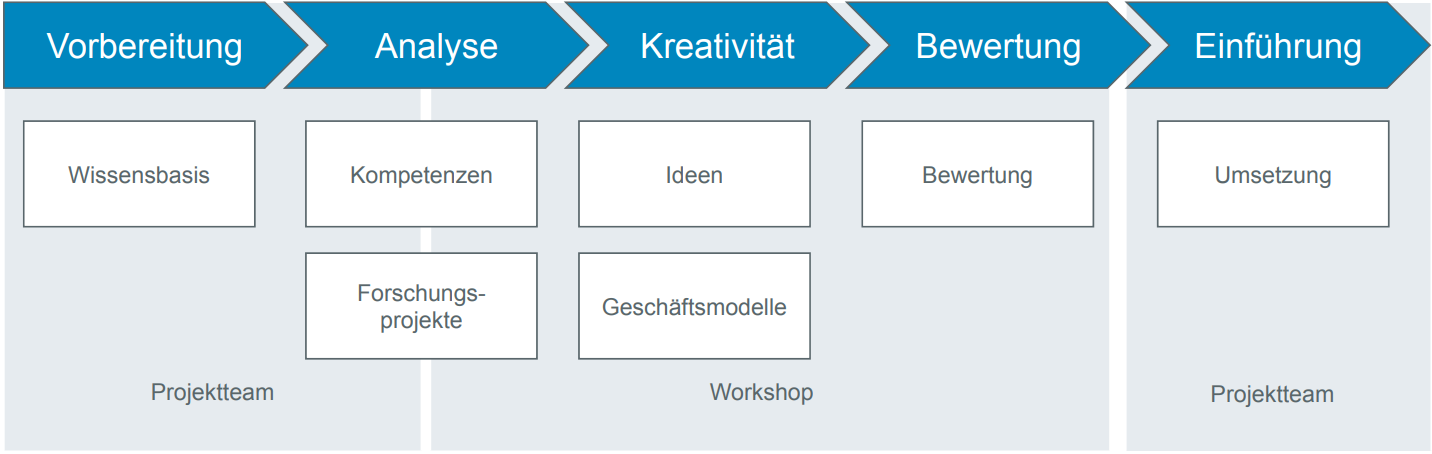
\includegraphics[width=1\linewidth]{Bilder/A5_VDMA_Phasen}
	\caption{Die fünf Phasen des VDMA Leitfadens für Industrie 4.0 \cite[S.10]{2}}
	\label{fig:VDMAAufbauLeitfaden}
\end{figure}
\begin{enumerate}
	\item \textbf{„Vorbereitungsphase"} \cite[S.10]{2} \\ In der ersten Phase soll eine Wissensbasis für alle Teilnehmer geschaffen werden. Das Unternehmen soll Kenntnisse über den Markt und über ihr eigenes Produkt aufbauen. Diese grundlegende Wissensbasis ist der „Ausgangspunkt für die Erarbeitung von Produktideen und Verbesserungen in der internen Produktion“ \cite[S.10]{2}.
	\item \textbf{„Analysephase"} \cite[S.10]{2} \\ In der zweiten Phase werden die Kompetenzen des Unternehmen im Bereich von Industrie 4.0 Technologien untersucht. Die Kompetenzen des Unternehmens werden sowohl produktseitig als auch produktionsseitig untersucht. Diese Phase liefert eine „Ausgangsbasis für die spätere Ideengenerierung“ \cite[S.10]{2}.
	\item \textbf{„Kreativitätsphase"} \cite[S.10]{2} \\ In der dritten Phase geht es um die „Generierung neuer Ideen und die anschließende Ausarbeitung von Konzepten für Geschäftsmodelle“\cite[S.10]{2}, basierend auf dem aufgebauten Wissen der vorherigen zwei Phasen \cite[S.10]{2}.
	\item \textbf{„Bewertungsphase"} \cite[S.10]{2} \\ In der vierten Phase werden die zuvor erarbeiteten Konzepte bewertet um Geschäftsmodelle „mit hohem Potential bei geringen Ressourceneinsatz“ \cite[S.10]{2} zu identifizieren \cite[S.10]{2}.
	\item \textbf{„Einführungsphase"} \cite[S.10]{2} \\ In der fünften und letzten Phase geht es um die Ausarbeitung der gesammelten Konzepte, damit diese „in entsprechende Projekte überführt und vorangetrieben“ \cite[S.10]{2} werden können \cite[S.10]{2}.
\end{enumerate}
Zentrales Element des Leitfadens ist der sogenannte „Werkzeugkasten Industrie 4.0“, der in  Abbildung \ref{fig:VDMAWerkzeugkasten} zu sehen ist. Der Werkzeugkasten „zeigt Entwicklungsstufen für verschiedene Anwendungsebenen von Industrie 4.0 auf“ \cite[S.11]{2} und soll bei der „schrittweisen Umsetzung innovativer Ideen in kleinen und mittelständischen Unternehmen“ behilflich sein \cite[S.11]{2}. Dabei ist der Werkzeugkasten unterteilt in zwei Hälften: Produkte und Produktion. Die einzelnen Entwicklungsstufen auf jeder Anwendungsebene sind in steigender Komplexität von links nach rechts sortiert. Es ist anzumerken, dass der Werkzeugkasten weiterentwickelt werden muss, da „die Entwicklungen der vierten industrielle Revolution noch lange nicht abgeschlossen“ \cite[S.11]{2} sind und daher einige „technologische Entwicklungsstufen nicht umfänglich vorausgesagt werden können“ \cite[S.11]{2}.
\begin{figure}[h]
	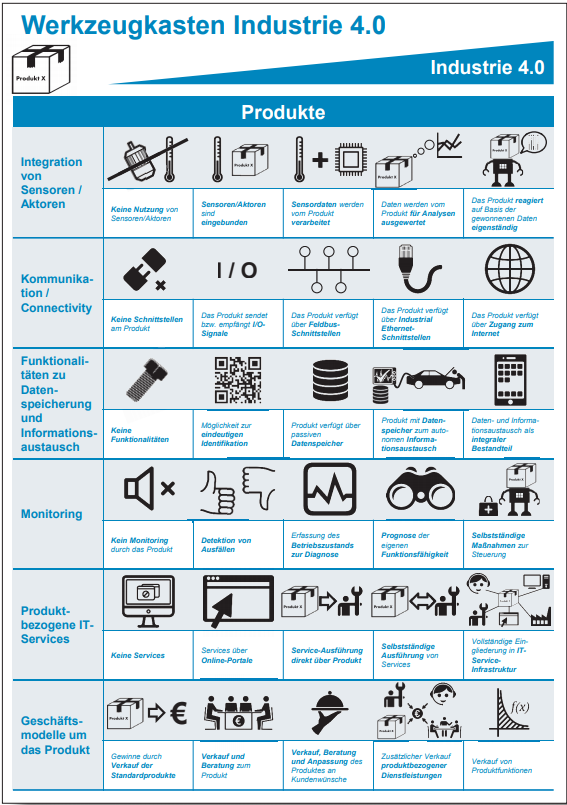
\includegraphics[width=0.5\linewidth]{Bilder/A6_VDMAWerkzeugkasten1}
	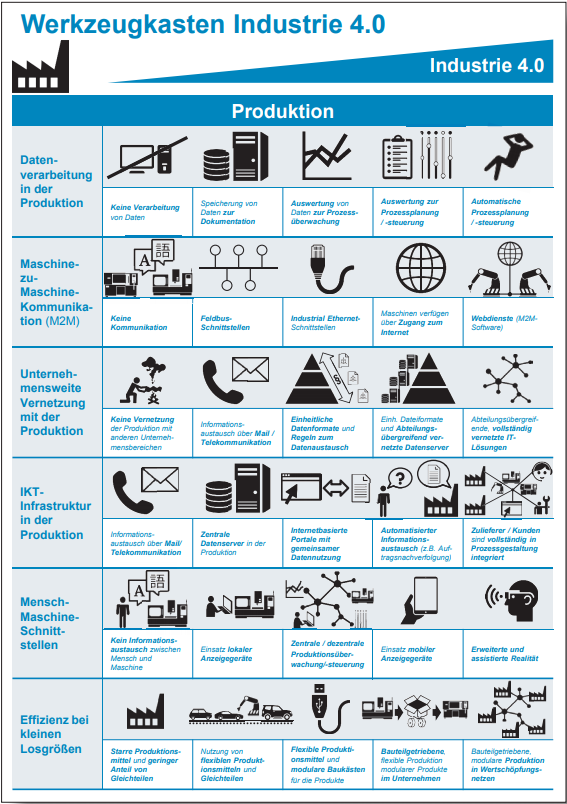
\includegraphics[width=0.499\linewidth]{Bilder/A7_VDMAWerkzeugkasten2}
	\caption{Der Werkzeugkasten des VDMA Leitfadens für Industrie 4.0 \cite[S.9]{2}}
	\label{fig:VDMAWerkzeugkasten}
\end{figure}
\newline
\noindent Der Bereich der Produkte befasst sich mit der Frage, inwiefern sich mit Hilfe von Industrie 4.0 Produkte entwickeln (oder auch weiterentwickeln) lassen können, sodass diese für Kunden einen Mehrwert liefern. Auf der Seite der Produkte umfasst der Werkzeugkasten folgende Anwendungsebenen \cite[S.13]{2}:
\begin{enumerate}
	\item \textbf{„Integration von Sensoren und Aktoren"} \cite[S.13]{2} \\ Die Entwicklungen auf dieser Anwendungsebene reichen von Produkten mit keinen Sensoren/Aktoren, bis zu intelligenten Produkten die auf Basis der gewonnen Daten eigenständig reagieren und mit den Cyber-physischen-Systemen kommunizieren können \cite[S.13]{2}.
	\item \textbf{„Kommunikation und Konnektivität"} \cite[S.13]{2} \\ Die Entwicklungen auf dieser Anwendungsebene reichen von Produkten, die keine Schnittstelle zur Außenwelt besitzen, bis hin zu Produkten die über eine Anbindung zum Internet verfügen \cite[S.13]{2}.
	\item \textbf{„Funktionalitäten zur Datenspeicherung und dem Informationsaustausch"} \cite[S.13]{2} \\ Die Entwicklungen auf dieser Anwendungsebene reichen von Produkten, die keine Funktionalitäten zur Datenspeicherung und Informationsaustausch besitzen, bis hin zu Produkten bei denen dies ein integraler Bestandteil ist \cite[S.13]{2}.
	\item \textbf{„Monitoring"} \cite[S.13]{2} \\ Die Entwicklungen auf dieser Anwendungsebene reichen von Produkten, die kein eigenständiges Monitoring durchführen können, bis hin zu Produkten die selbstständig die Steuerung der Produktion übernehmen können \cite[S.13]{2}.
	\item \textbf{„Produktbezogene IT-Services"} \cite[S.13]{2} \\ Die Entwicklungen auf dieser Anwendungsebene reichen von Produkten, die keine zusätzlichen Dienstleistungen anbieten, bis hin zu Produkten die vollständig eingegliedert sind in eine übergeordnete IT-Service-Infrastruktur \cite[S.13]{2}.
	\item \textbf{„Geschäftsmodelle um das Produkt"} \cite[S.13]{2} \\ Die Entwicklungen auf dieser Anwendungsebene reichen von Produkte, bei denen der Gewinn nur durch den Verkauf der Produkte gemacht wird, bis hin zu Produkten bei denen Gewinn durch den Verkauf zusätzlicher Produktfunktionen (z.B. Dienstleistungen) gesteigert wird \cite[S.13]{2}.
\end{enumerate}
Im Bereich der Produktion beschäftigt man sich mit der Frage, wie Industrie 4.0 es den Unternehmen ermöglichen kann, dass sowohl Produktionsabläufe optimiert, als auch Produktionskosten gesenkt werden. Auf der Seite der Produktion umfasst der Werkzeugkasten folgende Anwendungsebenen \cite[S.15]{2}:
\begin{enumerate}
	\item \textbf{„Datenverarbeitung in der Produktion"} \cite[S.15]{2} \\ Die Entwicklungen auf dieser Anwendungsebene reichen von Produktionsanlagen, die keine Daten verarbeiten, bis hin zu Produktionsanlagen mit automatisierten Prozessplanungen und Steuerungen \cite[S.15]{2}.
	\item \textbf{„Maschine-zu-Maschine-Kommunikation (M2M)"} \cite[S.15]{2} \\ Die Entwicklungen auf dieser Anwendungsebene reichen von Produktionsanlagen, die keine Form von Kommunikation zwischen Maschinen ermöglichen, bis hin zu Produktionsanlagen die durch eine Internet-Schnittstelle eingebunden sind in Webdienste (Cloud) \cite[S.15]{2}.
	\item \textbf{„Unternehmensweite Vernetzung mit der Produktion"} \cite[S.15]{2} \\ Die Entwicklungen auf dieser Anwendungsebene reichen von Produktionsanlagen, bei denen die Produktion nicht mit anderen Unternehmensbereichen vernetzt ist, bis hin zu Unternehmen die eine abteilungsübergreifende vernetzte IT-Infrastruktur besitzen \cite[S.15]{2}.
	\item \textbf{„IKT-Infrastruktur in der Produktion"} \cite[S.15]{2} \\ Die Entwicklungen auf dieser Anwendungsebene reichen von Produktionsanlagen, bei denen der gesamte Informationsaustausch über Telefon oder E-Mail stattfindet, bis hin zu Unternehmen bei denen die Zulieferer und Kunden in der Prozessgestaltung berücksichtigt werden. \cite[S.15]{2}.
	\item \textbf{„Mensch-Maschine-Schnittstellen"} \cite[S.15]{2} \\ Die Entwicklungen auf dieser Anwendungsebene reichen von Produktionsanlagen, deren Maschinen keinen direkten Informationsaustausch mit den Menschen ermöglichen, bis hin zu Produktionsanlagen bei denen die Mitarbeiter mit Hilfe von erweitertet und assistierter Realität direkt Informationen von den Maschinen auslesen können \cite[S.15]{2}.
	\item \textbf{„Effizient bei kleinen Losgrößen"} \cite[S.15]{2} \\ Die Entwicklungen auf dieser Anwendungsebene reichen von Produktionsanlagen, die nicht dynamisch und somit ineffizient bei kleinen Losgrößen sind, bis hin zu modularen in Wertschöpfungsnetzen integrierten Produktionen, bei denen verschiedene Anlagen die Einzelteile fertigen \cite[S.15]{2}.
\end{enumerate}
Für diese Arbeit ist die Anwendungsebene „Mensch-Maschine-Schnittstelle“ auf der Produktionsseite des Werkzeugkastens am relevantesten, da der Einsatz von erweiterter Realität (Virtual Reality) die Kommunikation zwischen Mensch und Maschine maßgeblich verändern wird. Diese Entwicklung ermöglicht einige neue Geschäftsmodelle im Bereich von Industrie 4.0, wie z.B. die standortunabhängige Interaktion mit Produktionsanlagen mit Hilfe von Virtual Reality Brillen.

\subsubsection{Leitbild 2030 für Industrie 4.0 - Digitale Ökosysteme global gestalten}\label{sec:PlattformIndustrieLeitfaden}
Dieser Leitfaden stellt, im Gegensatz zu dem vorher vorgestellten Leitfaden, den Unternehmen keinen Werkzeugkasten zur Verfügung. Stattdessen konzentriert sich der Leitfaden auf die drei Handlungsfelder Souveränität, Interoperabilität und Nachhaltigkeit. Laut den Verfassern dieses Leitfadens sind diese Handlungsfelder eng miteinander verknüpft und bilden die zentralen und strategischen Bausteine für eine erfolgreiche Umsetzung von Industrie 4.0. Des Weiteren sehen die Verfasser die genannten Handlungsfelder als „leitend für die kommende Dekade der anstehenden Skalierung von Industrie 4.0 in Deutschland, Europa und weltweit“ \cite[S.3]{3} an.

\paragraph{Souveränität}\label{sec:Souveränität}
\noindent Souveränität soll die „Freiheit alles Akteure am Markt (Unternehmen, Mitarbeiter, Wissenschaft, Einzelpersonen) selbstbestimmte, unabhängige Entscheidungen zu treffen“ \cite[S.4]{3} gewährleisten um somit einen fairen Wettbewerb zu ermöglichen \cite[S.4]{3}. Souveränität erfordert:
\begin{enumerate}
	\item \textbf{„Digitale Infrastruktur"} \cite[S.4]{3} \\
	Es wird eine über Unternehmensgrenzen hinweg reichende leistungsstarke und souveräne
	Infrastruktur benötigt. „Diese Infrastruktur muss für alle Teilnehmer gleichermaßen offen 
	zugänglich sein und ohne Einschränkungen zur Verfügung stehen“ \cite[S.4]{3}.
	\item \textbf{„Sicherheit"} \cite[S.4]{3} \\
	„Datenschutz, IT- und Informationssicherheit stellen einen fest etablierten industriellen
	und gesellschaftlichen Wert dar“ \cite[S.4]{3} und sind somit „eine Grundvoraussetzung
	für Industrie 4.0 und die Kooperation innerhalb digitaler Ökosysteme“ \cite[S.4]{3}.
	\item \textbf{„Technologieentwicklung"} \cite[S.4]{3} \\
	Der Fortschritt von Industrie 4.0 basiert auf „Forschung, Entwicklung und Innovationen“ 
	\cite[S.4]{3}, daher sollen alle Teilnehmer am Wettbewerb „an den technologischen 
	Entwicklungen partizipieren und profitieren“ \cite[S.4]{3}.
\end{enumerate}

\paragraph{Interoperabilität}\label{sec:Interoperabilität}
\noindent Ein zentraler Bestandteil der Industrie 4.0 ist die „flexible Vernetzung unterschiedlicher Akteure“ \cite[S.5]{3}. Um eine Vernetzung zwischen vielen verschieden Akteuren zu gewährleisten, ist die Interoperabilität eine Schlüsselkomponente. Es wird vorausgesetzt, dass alle Teilnehmer sich an die Standards zur Interoperabilität einhalten, aktiv zu der Entwicklung dieser Standards beitragen und somit eine „Vernetzung über Unternehmens- und Branchengrenzen hinweg“ \cite[S.5]{3} ermöglichen \cite[S.5]{3}. Interoperabilität erfordert:
\begin{enumerate}
	\item \textbf{„Standards und Integration"} \cite[S.5]{3} \\
	Standards stellen die „Basis für die Interoperabilität dar" \cite[S.5]{3} und erleichtern die Integration von neunen Komponenten. Das Entwickeln von branchenübergreifenden Standards und
	Referenzarchitekturen ist jedoch aufwendig \cite[S.5]{3}.
	\item \textbf{„Regulatorischer Rahmen"} \cite[S.5]{3} \\
	Ein regulatorischer Rahmen ist notwendig, um für alle Akteure am Markt faire Bedingungen zu gewährleisten \cite[S.5]{3}.
	\item \textbf{„Dezentrale Systeme und Künstliche Intelligenz"} \cite[S.5]{3} \\
	Dezentrale Systeme und künstliche Intelligenz sind für die industrielle Wertschöpfung im 
	B2B-Bereich „von sehr viel größerer Bedeutung als im B2C-Bereich" \cite[S.5]{3}. Die Nutzung,
	Verknüpfung und Auswertung von großen Datenmengen erfordert ein gut vernetztes Ökosystem. Um Künstliche Intelligenz sinnvoll einsetzen zu können, muss „neben Big Data vor allem die Gewinnung und Nutzung von Smart Data“ \cite[S.5]{3} ermöglicht werden.
\end{enumerate}

\paragraph{Nachhaltigkeit}\label{sec:Nachhaltigkeit}
\noindent Nachhaltigkeit ist von zentraler Bedeutung für den Wandel zu Industrie 4.0, denn „ökonomische, ökologische und soziale Nachhaltigkeit stellen einen fundamentalen Eckpfeiler der gesellschaftlichen Wertorientierung dar“ \cite[S.6]{3}. Des Weiteren trägt die Nachhaltigkeit „entscheidend zur Erhaltung des Lebensstandards der Gesellschaft bei“ \cite[S.6]{3}.
Nachhaltigkeit erfordert:
\begin{enumerate}
	\item \textbf{„Gute Arbeit und Bildung"} \cite[S.6]{3} \\
	Um Beschäftigungsniveau hoch zu halten und wettbewerbsfähig zu bleiben, müssen
	Weiterbildungsmöglichkeiten geschaffen werden \cite[S.6]{3}.
	\item \textbf{„Gesellschaftliche Teilhabe"} \cite[S.6]{3} \\
	Da Industrie 4.0 „einen gesamtgesellschaftlichen Transformationsprozess“ \cite[S.6]{3} darstellt, erfordert der Wandel die „Beteiligung und Mitbestimmung aller Akteure" \cite[S.6]{3}.
	\item \textbf{„Klimaschutz"} \cite[S.6]{3} \\
	Um den Klimaschutz zu gewährleisten bedarf es einer steigenden Ressourceneffizienz
	und einem besseren Recycling von Stoffen \cite[S.6]{3}.
\end{enumerate}
%--------------------------------------------------------------------------------------------------
\section{Die Ausgangslage der industriellen Fertigung}\label{sec:IndustrielleFertigung}
Dieses Kapitel behandelt die Ausgangslage der industriellen Fertigung. Daher gibt es zunächst einen Einblick in den Produktlebenszyklus und die Automatisierungspyramide der industriellen Fertigung, bevor im Anschluss die Wandlung der Automatisierungspyramide im Kontext von Industrie 4.0 erläutert wird.

\subsection{Der Produktlebenszyklus}\label{sec:Produktlebenszyklus}
\begin{figure}[h]
	\centering
	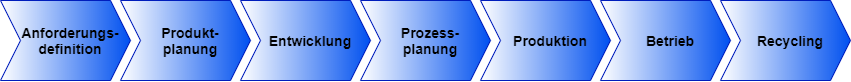
\includegraphics[width=1\linewidth]{Bilder/A8_Produktlebenszyklus}
	\caption{Der Produktlebenszyklus, Abbildung nach \cite[S.3]{13}}
	\label{fig:Produktlebenszyklus}
\end{figure}
\noindent Der Produktlebenszyklus umfasst wie in Abbildung \ref{fig:Produktlebenszyklus} zu sehen ist insgesamt sieben Phasen und reicht von der Anforderungsdefinition bis zum Recycling. Auffällig dabei ist, dass der Produktlebenszyklus neben den unternehmensinternen Phasen bis hin zur Produktion auch die Phasen „Betrieb“ und „Recycling“ enthält. Somit ist der Produktlebenszyklus ein interdisziplinärer Prozess und bildet strenggenommen keinen Zyklus, sondern den Lebenslauf eines Produktes ab \cite[S.3]{13}.
\newline
Für diese Arbeit sind die Phasen Prozessplanung und Produktion am relevantesten, da der Einsatz von erweiterter Realität (Virtual Reality) in Verbindung mit einem Menschmodell (steuerbares virtuelles Abbild eines Menschen) neue Geschäftsmodelle in diesem Bereich ermöglichen wird. Dazu gehören Beispielsweise die Produktionsplanung oder die Fernsteuerung von Produktionsanlagen über einen virtuellen Zwilling.

\subsection{Die Automatisierungspyramide}\label{sec:Automatisierungspyramide}
Die Automatisierungspyramide aus Abbildung \ref{fig:Automatisierungspyramide} hat aufgrund der zunehmenden „Automatisierung der Produktion die Aufgabe, die Komplexität der industriellen Fertigung durch die Unterteilung der anfallenden Prozesse, zur Datenerhebung und -verarbeitung, in einzelne ebenen zu verringen“ \cite[S.49]{14}. Sie ist besteht aus sechs aufeinander aufbauenden Stufen, die „die verschiedenen Ebenen der automatisierten Fertigung in einem Unternehmen“ \cite[S.49]{14} darstellen sollen. Es ist anzumerken, dass es zwischen den Siebzigern und Neunzigern einige Veränderungen in der Zusammensetzung der Automatisierungspyramide gab, sodass man auch davon ausgehen kann, dass es in Zukunft durchaus noch einige Veränderungen geben könnte \cite[S.49]{14}. Das Ziel der Automatisierungspyramide ist es, eine „leichtverständliche, visuelle Darstellung der industriellen Fertigung“ \cite[S.49]{14} zu sein und gleichzeitig die fließenden Übergänge der verschiedenen Ebenen innerhalb der Produktion hervorzuheben \cite[S.49]{14}.
\begin{figure}[h]
	\centering
	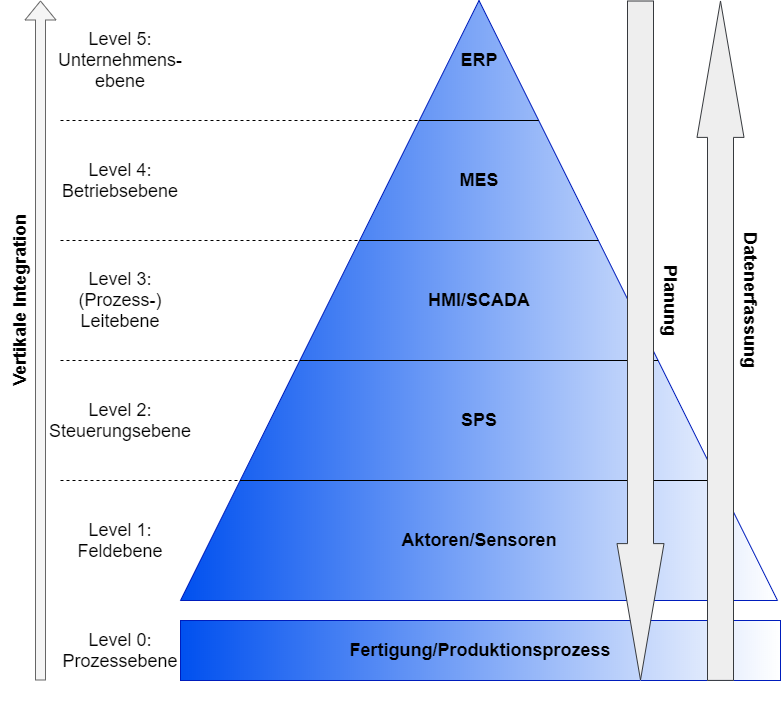
\includegraphics[width=1\linewidth]{Bilder/A9_Automatisierungspyramide}
	\caption{Die Automatisierungspyramide, Abbildung nach \cite[S.49]{14}}
	\label{fig:Automatisierungspyramide}
\end{figure}
\newline\newline
\noindent Die einzelnen Ebenen der Automatisierungspyramide lauten:
\begin{enumerate}
	\item \textbf{„Prozessebene"} \cite[S.49]{14} \\
	Die unterste Ebene, die Prozessebene, befasst sich mit der Fertigung und dem eigentlichen Produktionsprozess \cite[S.49]{14}. Hier werden Daten, die meistens in Form von binären Signalen vorliegen, durch die Maschinen gesammelt \cite[S.405]{15}. Das Sammeln dieser Daten wird z.B. durch intelligente Produkte mit integrierten RFID-Chips (Radio Frequency Identification-Chips) ermöglicht \cite[S.49]{14}.
	\item \textbf{„Feldebene"} \cite[S.50]{14} \\
	Die Feldebene liefert die Informationen über die Produktionsstätte und beinhaltet Sensoren (z.B. Temperaturfühler, Lichtschranken, etc.). Des Weiteren verfügt diese Ebene über Aktoren (z.B. elektrische Regler, etc.). Zusammengefasst stellt diese Ebene die „technische Schnittstelle zum Produktionsprozess dar“ \cite[S.405]{15}. Zusammengefasst handhabt diese Ebene „Daten in Form von Ein- und Ausgangssignalen“ \cite[S.50]{14}.
	\item \textbf{„Steuerungsleitebene"} \cite[S.50]{14} \\
	Auf der Steuerungsebene findet die Auswertung von Eingangssignalen (Sensordaten) "über speicherprogrammierbare Steuerungen (SPS)" \cite[S.50]{14} statt. Des Weiteren werden „entsprechende Ergebnisdaten (Ausgangsignale) an die Feldebene zurück“ \cite[S.50]{14} gesendet. Die gesammelten Daten können verarbeitet und in mechanische Bewegungen (z.B. mit Druckluft oder Hydraulik) umgewandelt werden \cite[S.50]{14}. Diese Ebene stellt eine Schlüsselkomponente „zur Umsetzung einer dezentral gesteuerten Maschinen- und Anlagesteuerung“ \cite[S.50]{14} dar.
	\item \textbf{„(Prozess-) Leitebene"} \cite[S.50]{14} \\
	Zentrales Element der (Prozess-) Leitebene ist das SCADA (Supervisory Control and Data Acquisition). Auf der (Prozess-) Leitebene werden die Messwerte der untergeordneten Schichten gesammelt \cite[S.405]{15}. Des Weiteren ist die Ebene zuständig für die „Visualisierung produktionsrelevanter Vorgänge“ \cite[S.50]{14} und stellt somit eine Mensch-Maschine-Schnittstelle (HMI) dar. Sie ermöglicht das Monitoring (Bedienen und Beobachten) des ganzen Systems \cite[S.405]{15}.
	\item \textbf{„Betriebsebene"} \cite[S.50]{14} \\
	Auf der Betriebsebene übernimmt das MES (Manufacturing Execution System) „die Steuerung, Lenkung und Kontrolle der Produktion“ \cite[S.50]{14}. Die Ebene hat die Funktion eines Bindeglieds zwischen der Ebene der Maschinensteuerung und der Unternehmensebene \cite[S.50]{14}. Zu den Hauptaufgaben dieser Ebene gehören: Produktionsfeinplanung, Produktionsdatenerfassung und die Weitergabe von Planungsdaten an das ERP-System (Enterprise Resource Planning System) \cite[S.50]{14}.  Zusätzlich findet auf dieser Ebene die Überwachung der PKIs (Key Performance Indicators) und „das Material und Qualitätsmanagement statt" \cite[S.405]{15}.
	\item \textbf{„Unternehmensebene"} \cite[S.50]{14} \\
	Das vorher erwähnte ERP-System ist Bestandteil der Unternehmensebene, dessen Aufgabe „die Produktionsgrobplanung und Bestellabwicklung der industriellen Fertigung“ \cite[S.50]{14} ist. Des Weiteren wird die Unternehmensebene manchmal auch „Topfloor“ genannt \cite[S.50]{14}.
\end{enumerate}
Zusammenfassend ist es wichtig zu erwähnen, dass die einzelnen Ebenen nur mit direkt benachbarten Ebenen kommunizieren können. Außerdem kommen die Planung und die Datenerfassung aus unterschiedlichen Richtungen. Die Planung fängt ganz oben auf der Unternehmensebene an und geht bis nach ganz unten bis zur Prozessebene. Die Datenerfassung fängt ganz unten auf der Prozessebene an und geht dann über alle Ebenen hinweg bis zur Unternehmensebene \cite[S.50]{14}. Ein weiterer maßgeblicher Unterschied zwischen den Ebenen sind die Reaktionszeiten. Die Reaktionszeit auf der Unternehmensebene kann mehrere Monate betragen, während es auf den unteren Ebenen wie der Feldebene oder Prozessebene um Millisekunden geht \cite[S.123]{16}.
\newline\newline
Das Thema dieser Arbeit lässt sich am besten in die Betriebsebene einordnen, da auf dieser Ebene sowohl die Steuerung als auch die Produktionsfeinplanung stattfinden. Zusätzlich ermöglicht der Einsatz von erweiterter Realität (Virtual Reality) und digitalen Zwillingen von Produktionsstätten eine bessere Vernetzung zwischen der Betriebsebene und der Unternehmensebene.

\subsection{Automatisierungspyramide und Industrie 4.0}\label{sec:AutomatisierungspyramideUndIndustrie4.0}
Durch den Wandel zu Industrie 4.0 werden Cyber-Physical Production Systems (CPPS) zunehmend an Bedeutung gewinnen. CPPS sind gekennzeichnet durch den hohen Vernetzungsgrad und die durchgehende Verfügbarkeit aller Daten. Langfristig werden flexible und selbstorganisierte CPPS die Produktion „durch geringere Rüstzeiten und optimierten Energie- und Ressourceneinsatz" \cite[S.3]{17} effizienter, kostengünstiger und ressourcenschonender gestalten \cite[S.3]{17}.
\newline\newline
Ein wichtiges Merkmal von CPPS ist die Tatsache, dass durch den Einsatz von CPPS die „Daten, Dienste und Funktionen dort gehalten abgerufen und ausgeführt“ \cite[S.4]{17} werden, „wo es im Sinne einer flexiblen, effizienten Entwicklung (inkl. Entwurf und Engineering) und Produktion den größten Vorteil bringt“ \cite[S.4]{17}. In Zukunft müssen also die einzelnen Ebenen der Automatisierungspyramide nicht mehr eingehalten werden, da die Daten von den verschiedenen Ebenen Beispielsweise in eine Cloud ausgelagert werden können \cite[S.4]{17}.
\newline\newline
Aufgrund der zunehmenden Auslagerung in die Cloud geht man davon aus, dass sich die klassische Automatisierungspyramide „durch die Einführung von vernetzten, dezentralen Systemen“ \cite[S.4]{17} in Zukunft Schritt für Schritt auflösen wird, wie es in Abbildung \ref{fig:AutomatisierungspyramideCPPS} illustriert wird. Echtzeitkritische Steuerungen werden aber zunächst weiterhin auf der Feldebene bleiben, sofern es in der Zukunft keine technologischen Fortschritte gibt, die es ermöglichen auch diese Ebene in die Cloud auszulagern \cite[S.4]{17}.
\begin{figure}[h]
	\centering
	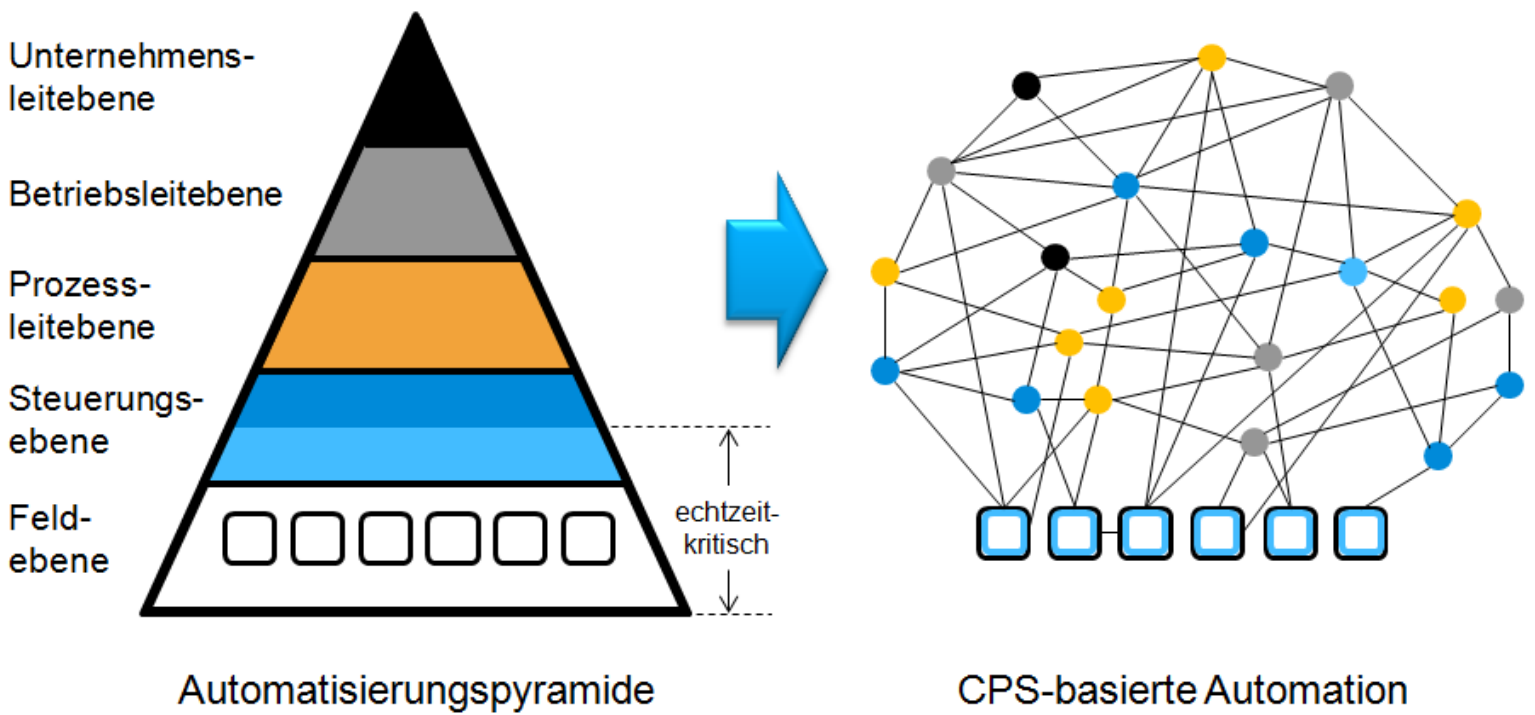
\includegraphics[width=1\linewidth]{Bilder/A10_AutomatisierungspyramideCPPS}
	\caption{Die Auflösung der Automatisierungspyramide \cite[S.4]{17}}
	\label{fig:AutomatisierungspyramideCPPS}
\end{figure}
\newline
\noindent Es ist besonders wichtig hervorzuheben, dass die Bedeutung von Mensch-Maschine-Schnittstellen zunehmen wird, da die Daten nicht mehr an einzelne Ebenen gebunden sein werden. Relevante Informationen aus dem Netzwerk zu Filtern und den Bedienern in geeigneter Form darzustellen wird eine große Herausforderung darstellen \cite[S.4]{17}.

%--------------------------------------------------------------------------------------------------
\section{Virtual Reality}\label{sec:VR}
Virtual Reality (deutsch: virtuelle Realität) beschreibt eine computergenerierte virtuelle Realität. Diese durch Computer geschaffene dreidimensionale virtuelle Realität wird auf zweidimensionalen Bildschirmen abgebildet. Es gibt unterschiedliche Arten um virtuelle Realitäten abzubilden, doch die weitverbreitetste Art sind sogenannte Virtual Reality Brillen (kurz: VR-Brillen). VR-Brillen werden im englischen auch abgekürzt durch die Begriffe VR-Headset (Virtual Reality Headset) und HMD (Head-Mounted-Display) \cite{19}.

\subsection{Die Geschichte von Virtual Reality}\label{sec:VRGeschichte}
\begin{figure}[h]
	\centering
	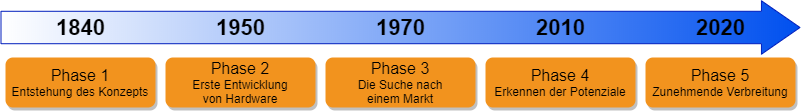
\includegraphics[width=1\linewidth]{Bilder/A12_GeschichteVR}
	\caption{Die Geschichte von Virtual Reality, eigene Abbildung nach \cite{20,21,22,23}}
	\label{fig:GeschichteVR}
\end{figure}
\noindent Wie es in Abbildung \ref{fig:GeschichteVR} illustriert wird, habe ich nach meiner Recherche die Geschichte von Virtual Reality in fünf Phasen aufgeteilt. Im Folgenden gibt es eine kurze Zusammenfassung der einzelnen Phasen. Es ist anzumerken, dass wir uns noch am Anfang der fünften Phase befinden. Daher ist es nicht möglich alle zukünftigen Entwicklungen vollständig vorherzusehen.

\subsubsection{Phase 1 - Entstehung des Konzepts}
1838 beschrieb Sir Charles Wheatstone als erster das Konzept Stereopsis (räumliches sehen) und erhielt dafür zwei Jahre später sogar eine Auszeichnung von der Royal Society. Seine Forschungen zeigten, dass das Menschliche Gehirn die unterschiedlichen Bilder beider Augen zu einem Bild kombiniert, um das räumliche Sehen zu ermöglichen. Aufgrund seiner Forschungen erfand er das Stereoskop (Abbildung \ref{fig:Stereoskop}), ein optisches Gerät zum Betrachten räumlicher Bilder. Die Augen des Betrachters werden zentral vor zwei Spiegeln positioniert die jeweils in einem 45 Grad Winkel zum Betrachtungswinkel stehen und Bilder reflektieren, die vom Betrachter aus jeweils Links und Rechts auf der Höhe der Spiegel positioniert werden \cite{20}.
\begin{figure}[h]
	\centering
	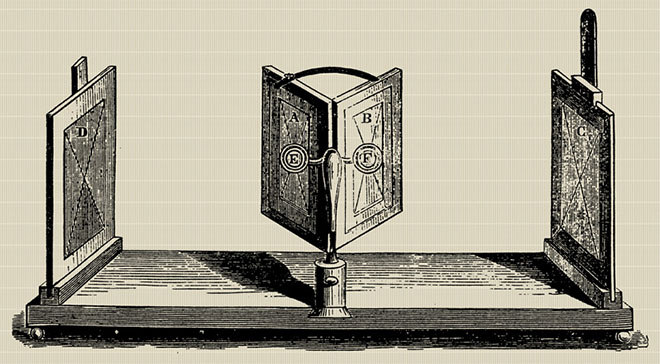
\includegraphics[width=0.5\linewidth]{Bilder/A13_Stereoskop}
	\caption{Stereoskop von Sir Charles Wheatstone \cite{20}}
	\label{fig:Stereoskop}
\end{figure}
\newline
\noindent
Einige Jahre Später, im Jahr 1935, veröffentlichte der Amerikanische Science-Fiction Autor Stanley Weinbaum eine Geschichte mit dem Namen „Pygmalion’s Spectacles“. In der Geschichte taucht der Protagonist durch eine Brille in eine fiktionale Welt ein, die nicht von der realen Welt zu unterscheiden ist. Diese Brille ist sogar in der Lage die menschlichen Sinne (Sehen, Hören, Riechen, Schmecken und Fühlen) zu stimulieren. Dies wird von vielen als der Ursprung vom Konzept der Virtual Reality gesehen \cite{20}.

\subsubsection{Phase 2 - Erste Entwicklung von Hardware}
Im Jahr 1956 entwickelte der Kameramann Morton Heilig das sogenannte „Sensorama“ (Vgl. Abbildung \ref{fig:SensoramaTelesphereSword}). Diese Große Kabine wird als die erste VR-Maschine betrachtet. Das Sensorama war eine große stationäre Maschine, die in der Lage war 3D Video in Farbe und Audio wiederzugeben. Des Weiteren konnte die Maschine Vibrationen, Wind, atmosphärische Effekte und sogar Gerüche Simulieren. Heilig sah in dieser Maschine die Zukunft des Kinos und es wurden sogar sechs kurze Filme dafür entwickelt \cite{20}.
\newline
Vier Jahre Später, im Jahr 1960, präsentierte Heilig seine „Telesphere Mask“ (Vgl. Abbildung \ref{fig:SensoramaTelesphereSword}), das erste HMD. Dies war jedoch nur dazu in der Lage, stereoskopische 3D-Bilder und Stereo Sound, aber keine Videos wiederzugeben. Zu dieser Zeit gab es ebenfalls noch kein Motion Tracking in den HMDs \cite{20}.
\newline
Nur ein Jahr später Entwickelten 1961 die Ingenieure Comeau und Bryan der Philco Corporation das erste HMD mit Motion Tracking und sogar Video Wiedergabe. Dieses HMD wurde jedoch nur für militärische Zwecke konzipiert und sollte Soldaten ermöglichen sich mithilfe von Ferngesteuerten Kameras in gefährlichen Gebieten umsehen zu können. Das amerikanische Militär erkannte das Potential von VR-Technologie sehr früh und so wurde bereits 1966 der erste Flugsimulator von Thomas Furness für die Air Force entwickelt \cite{20}.
\newline
Erst im Jahre 1968 wurde von Ivan Sutherland und seinem Schüler Bob Sproull das erste VR-HMD mit dem Namen „The Sword of Damocles“ (Vgl. Abbildung \ref{fig:SensoramaTelesphereSword}) entwickelt. Dabei wurde das HMD nicht wie bei vorherigen Ansätzen mit einer Kamera, sondern mit einem Computer verbunden. Der Computer berechnete die Anzeige von verschiedenen 3D Modellen und reagierte auf die Kopfbewegungen des Nutzers. Dieses HMD wurde aber nie weiterentwickelt, da es zu schwer, groß und unbequem war und blieb somit nur ein Laborprojekt, welches nie die Öffentlichkeit erreichte \cite{20}.
\begin{figure}[h]
	\centering
	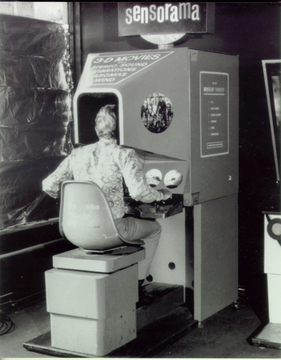
\includegraphics[width=0.22\linewidth]{Bilder/A14_Sensorama}
	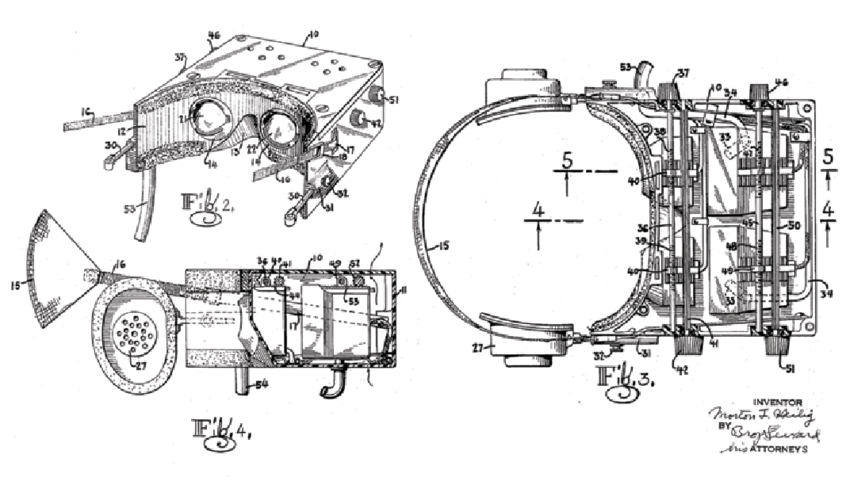
\includegraphics[width=0.3\linewidth]{Bilder/A15_TelesphereMask}
	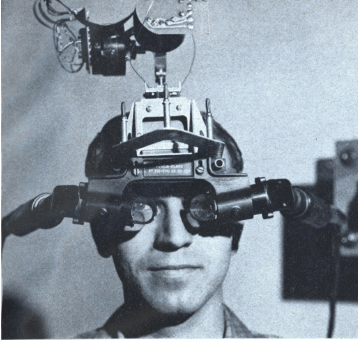
\includegraphics[width=0.3\linewidth]{Bilder/A16_SwordDamocles}
	\caption{Sensorama | Telesphere Mask | The Sword of Damocles \cite{A14,A15,A16}}
	\label{fig:SensoramaTelesphereSword}
\end{figure}

\subsubsection{Phase 3 - Die Suche nach einem Markt}
Über einen ziemlich langen Zeitraum hinweg gab es, bis auf den Einsatz in Militärtechnologie, keinen richtigen Verwendungszweck für VR-Technologie. Es gab viele verschiedene Ansätze, jedoch konnte sich kein Ansatz auf dem Markt durchsetzen. Im Folgenden werden ein paar Ansätze genauer erläutert.
\newline
Das MIT entwickelte 1977 ein VR-Ähnliches Programm, welches dem Nutzer ermöglichte sich, ähnlich wie heutzutage mit Google Street View, durch die Straßen von Aspen City in Colorado zu bewegen. Das Erlebnis war jedoch nur VR-Ähnlich, da normale Computer-Displays und keine HMDs eingesetzt wurden \cite{20}.
\newline
Einige Jahre später, im Jahr 1991, veröffentliche die Virtuality Group die erste VR Arcade Maschine namens „Virtuality“ (Vgl. Abbildung \ref{fig:VirtualityVRBoy}) für Spielehallen. Für diese VR Arcade Maschine erschienen, neben VR-Versionen von beliebten Spielen wie Pac-Man, sogar Spiele mit Multiplayer Funktionalität. Somit waren die VR Arcade Maschinen die ersten VR-Geräte, welche in die Massenproduktion gingen und erfolgreich vertrieben wurden \cite{20}.
\newline
Diesem Trend folgte unter anderem die Firma Nintendo und veröffentliche 1995 mit dem Virtual Boy (Vgl. Abbildung \ref{fig:VirtualityVRBoy}) die erste portable Spielekonsole in Form eines VR Headsets. Der Virtual Boy von Nintendo scheiterte jedoch aufgrund seines Schwarz-Weiß Displays und da nur sehr wenig Software dafür entwickelt wurde. Daher wurde die Produktion nach nur einem Jahr wieder eingestellt \cite{20}.
\newline
Zusammenfassend lässt sich sagen, dass in den Jahren zwischen 1990 und 2000 einige VR-Headsets veröffentlicht wurden, sich jedoch kein Headset durchsetzen konnte. Der Grund dafür werden höchstwahrscheinlich die Limitierungen der damaligen Hardware sein.
\begin{figure}[h]
	\centering
	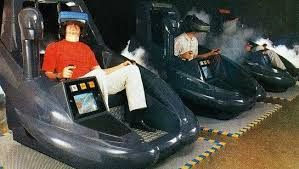
\includegraphics[width=0.4\linewidth]{Bilder/A17_Virtuality}
	\includegraphics[width=0.4\linewidth]{Bilder/A18_VIrtualBoy}
	\caption{Virtuality | Virtual Boy \cite{20, A18}}
	\label{fig:VirtualityVRBoy}
\end{figure}

\subsubsection{Phase 4 - Erkennen der Potenziale}
Die aktuellen Entwicklungen im Bereich der VR-Technologie lassen sich zum großen Teil auf das Jahr 2010 zurückführen.
\newline
In dem Jahr veröffentliche Google einen stereoskopischen 3D Modus für Ihre Anwendung Street View. Des Weiteren entwickelte Palmer Luckey, welcher zu dem Zeitpunkt gerade erst 18 Jahre alt war, in diesem Jahr seinen Prototyp vom Oculus Rift Headset. Beim Oculus Rift Headset wird die Berechnung der anzuzeigenden Bilder durch einen Computer übernommen. Luckey gründete daraufhin 2012 das Unternehmen Oculus VR und startete eine Crowd-Funding Kampagne über die Plattform Kickstarter, bei der er insgesamt 2,4 Millionen US-Dollar an Kapital von privaten Investoren sammeln konnte. Aufgrund dieser Entwicklungen steigerte sich das öffentliche Interesse für 3D- und VR-Technologie enorm \cite{20}.
\newline
Als zwei Jahre später, im Jahr 2014, der Technologie-Gigant Facebook die Firma Oculus VR für insgesamt 2 Milliarden US-Dollar kaufte, weckte dies das Interesse von weiteren Firmen, die Ihre eigenen VR-Brillen ankündigten. Diese Entwicklungen gaben dem Markt für VR-Technologien einen weiteren enormen Aufschwung \cite{20}.
\newline
Zu den Firmen, die eigene VR-Brillen ankündigten und/oder herausgebracht haben, gehören weitere Tech-Giganten wie Google, HTC, Microsoft, Samsung, Sony und viele weitere \cite{20}.

\subsubsection{Phase 5 - Zunehmende Verbreitung}
Wie bereits erwähnt befinden wir uns nach am Anfang der fünften Phase und es ist uns nicht möglich alle zukünftigen Entwicklungen und Einsatzzwecke von VR-Technologien vollständig vorherzusehen. Daher gibt es in Kapitel \ref{sec:VRPotentialUndAusblick} einen Einblick in die Potenziale von VR-Technologie.

\subsection{Potenziale von Virtual Reality }\label{sec:VRPotentialUndAusblick}
Visual Computing und damit auch die VR-Technolgie, wird als eine „Key Enabling Technology" \cite[S.1]{5} (Schlüsselkomponente) für die Realisierung von Industrie 4.0 angesehen.
Der Einsatz von VR-Technologie bringt eine Menge an Potenzialen, auch für den Einsatz außerhalb der Industrie mit sich. Im folgenden sind einige mögliche Anwendungsszenarien für VR-Technologie aufgelistet:
\begin{itemize}
	\item Produktionsanlagen in der virtuellen Realität begehen \cite{33}
	\item Materialfluss-Visualisierung durch Echtzeit-Simulationen in der virtuellen Realität \cite{33}
	\item Virtuelle Arbeitsplätze, mit Fokus auf Ergonomie und Effizienz \cite{33}
	\item Produkt- und Produktionsplanung in der virtuellen Realität \cite{33}
	\item Einsatz in der Medizin, z.B. für das Training von angehenden Ärzten \cite{23}
	\item Einsatz in der Lehre, z.B. für virtuelle Klassenausflüge \cite{23}
	\item Training von Polizei- und Feuerwehreinsatzkräften \cite{23}
	\item Virtuelle Meetings \cite{23}
\end{itemize}
Zusammenfassend lässt sich sagen, das VR-Technologien eine große Menge, von Teilweise noch unbekannten Potenzialen haben und durch die vielseitigen Einsatzmöglichkeiten maßgeblich bei der Umsetzung von Industrie 4.0 behilflich sein können.

%--------------------------------------------------------------------------------------------------